\section{Experiments}
\label{section:experiments}
\begin{table}
\begin{center}
    \begin{tabular}{cccccccc}
    \toprule
    \textbf{\#} & \textbf{S} &  & \textbf{M} & & \textbf{L} & & \textbf{XL} \\
    \midrule
    \textbf{Conv. Layers}      & 20 & & 30 & & 50& & 70 \\
    \textbf{Channels}  &45 & & 60 & & 90 & & 120 \\ 
    \textbf{Lin. Layers}        &7 & & 10 & & 15 & & 15 \\
    \textbf{Lin. Features} & 2048 & & 2048 & & 4096 & & 4096 \\
    \bottomrule
    \end{tabular}%

\end{center}
\caption{\label{table:model-desc}
Architectures description for our Convex Potential Layers (CPL) neural networks with different capacities. We vary the number of Convolutional Convex Potential Layers, the number of Linear Convex Potential Layers, the number of channels in the convolutional layers and the width of fully
connected layers. They will be reported respectively as CPL-S, CPL-M, CPL-L and CPL-XL.}
\end{table}

To evaluate our new $1$-Lipschitz Convex Potential Layers, we conducted an extensive set of experiments. In this section, we first describe  the details of our experimental setup. We then recall  the concurrent approaches that build $1$-Lipschitz Neural Networks and stress their limitations. Our experimental results are finally summarized in Section~\ref{sec:setting-xp}. By computing the certified and empirical adversarial  accuracy of our networks on CIFAR10 and CIFAR100 classification tasks~\citep{krizhevsky2009learning}, we show that our architecture is competitive with state-of-the-art methods (Sections~\ref{sec:results}). We also study the influence of some hyperparameters and demonstrate the stability and the scalability of our approach by training very deep neural networks up to 1000 layers without normalization tricks or gradient clipping.










\subsection{Training and Architectural Details}
\label{sec:setting-xp}

We demonstrate the effectiveness of our approach on a classification task with CIFAR10 and CIFAR100 datasets~\citep{krizhevsky2009learning}. We use a similar training configuration to the one proposed in~\citep{trockman2021orthogonalizing}.
We trained our networks with a batch size of $256$ over $200$ epochs.
We use standard data augmentation (i.e. random cropping and flipping), a learning rate of $0.001$ with Adam optimizer \citep{diederik2014adam} without weight decay and a piecewise triangular learning rate scheduler. We used a margin parameter in the loss set to $0.7$.

As other usual convolutional neural networks, we first stack few Convolutional CPLs and then stack some Linear CPLs for classification tasks. To validate the performance  and the scalability of our layers,  we  evaluate four different variations of different hyperparameters as described in Table~\ref{table:model-desc}, respectively named CPL-S, CPL-M, CPL-L and CPL-XL, ranked according to the number of parameters they have. In all our experiments, we made $3$ independent trainings to evaluate accurately the models. All reported results are the average of these $3$ runs.

\subsection{Concurrent Approaches} We compare our networks with SOC~\citep{skew2021sahil} and Cayley~\cite{trockman2021orthogonalizing} networks which are to our knowledge the best performing approaches for deterministic $1$-Lipschitz Neural Networks. Since our layers are fundamentally different from these ones, we cannot compare with the same architectures. We reproduced SOC results for with $10$ and $20$ layers, that we call respectively SOC-$10$ and SOC-$20$ in the same training setting, {i.e.} normalized inputs, cross entropy loss, SGD optimizer with learning rate $0.1$ and multi-step learning rate scheduler. For Cayley layers networks, we reproduced their best reported model, {i.e.} KWLarge with width factor of $3$. 

The work of~\citet{singla2021householder} propose three methods to improve certifiable accuracies from SOC layers: a new HouseHolder activation function (HH),  last layer normalization (LLN), and certificate regularization (CR). The code associated with this approach is not open-sourced yet, so we just reported the results from their paper in ours results (Tables~\ref{table:c10-comp} and~\ref{table:c100-comp}) under the name SOC+. We were being able to implement the LLN method in all models. This method largely improve the result of all methods on CIFAR100, so we used it for all networks we compared on CIFAR100 (ours and concurrent approaches).


\begin{table*}[tb]
  \centering
  \sisetup{%
    table-align-uncertainty=true,
    separate-uncertainty=true,
    detect-weight=true,
    detect-inline-weight=math
  }
  \begin{tabular}
  {
    l
    S[table-format=2.2]
    S[table-format=2.2]
    S[table-format=2.2]
    S[table-format=2.2]
    S[table-format=2.2]
  }
  \toprule
    & \multicolumn{1}{c}{\textbf{Standard Accuracy}} & \multicolumn{3}{c}{\textbf{Provable Accuracy ($\varepsilon $)}} &  \multicolumn{1}{c}{\textbf{Time per epoch (s)}} 
    \\
    \cmidrule{3-5}
    & \multicolumn{1}{c}{ } & \multicolumn{1}{c}{36/255} & \multicolumn{1}{c}{72/255} &  \multicolumn{1}{c}{108/255} & \multicolumn{1}{c}{\textbf{}} 
    \\
  \midrule
    \textbf{CPL-S} & 75.6  & 62.3  & 46.9  & 32.2  & 21.9 \\
  \textbf{CPL-M} & 76.8  & 63.3  & 47.5  & 32.5  & 40.0 \\
  \textbf{CPL-L} & 77.7  & 63.9 & 48.1 & 32.9  & 93.4 \\
  \textbf{CPL-XL} & 78.5  & 64.4  & 48.0  & 33.0 & 163 \\
  \midrule
  \textbf{Cayley (KW3)} & 74.6  & 61.4  & 46.4  & 32.1  & 30.8\\
    \midrule

  \textbf{SOC-10} & 77.6  & 62.0  & 45.0  & 29.5  & 33.4 \\
  \textbf{SOC-20} & 78.0  & 62.7 & 46.0  & 30.3  &52.2\\
  \midrule
    \textbf{SOC+-10} & 76.2 &62.6 & 47.7 & 34.2& N/A\\
  \textbf{SOC+-20} & 76.3&62.6& 48.7& 36.0& N/A \\

  \bottomrule
  \end{tabular}%
  \caption{Results on the CIFAR10 dataset on standard and  provably certifiable accuracies for different values of perturbations $\varepsilon$ on CPL (ours), SOC and Cayley models. The average time per epoch in seconds is also reported in the last column. None of these networks uses Last Layer Normalization.}
  \label{table:c10-comp}%
\end{table*}%

\begin{table*}[tb]
  \centering
  \sisetup{%
    table-align-uncertainty=true,
    separate-uncertainty=true,
    detect-weight=true,
    detect-inline-weight=math
  }
  \begin{tabular}
  {
    l
    S[table-format=2.2]
    S[table-format=2.2]
    S[table-format=2.2]
    S[table-format=2.2]
    S[table-format=2.2]
  }
  \toprule
    & \multicolumn{1}{c}{\textbf{Standard Accuracy}} & \multicolumn{3}{c}{\textbf{Provable Accuracy ($\varepsilon $)}} &  \multicolumn{1}{c}{\textbf{Time per epoch (s)}} 
    \\
    \cmidrule{3-5}
    & \multicolumn{1}{c}{ } & \multicolumn{1}{c}{36/255} & \multicolumn{1}{c}{72/255} &  \multicolumn{1}{c}{108/255} & \multicolumn{1}{c}{\textbf{}} 
    \\
  \midrule
    \textbf{CPL-S} & 44.0  & 29.9  & 19.1  & 11.0  & 22.4 \\
  \textbf{CPL-M} & 45.6  & 31.1  & 19.3  & 11.3 & 40.7 \\
  \textbf{CPL-L} & 46.7  & 31.8 & 20.1  & 11.7  & 93.8 \\
  \textbf{CPL-XL} & 47.8  & 33.4  & 20.9  &  12.6  & 164 \\
  \midrule
  \textbf{Cayley (KW3)} & 43.3  & 29.2  & 18.8 & 11.0  & 31.3 \\
    \midrule

  \textbf{SOC-10} & 48.2  & 34.3  &22.7 & 14.0  & 33.8 \\
  \textbf{SOC-20} & 48.3  & 34.4 & 22.7  & 14.2 & 52.7 \\
  \midrule
    \textbf{SOC+-10} & 47.1& 34.5& 23.5& 15.7& N/A \\
  \textbf{SOC+-20} & 47.8 & 34.8 & 23.7 & 15.8 &  N/A\\

  \bottomrule
  \end{tabular}%
  \caption{Results on the CIFAR100 dataset on standard and  provably certifiable accuracies for different values of perturbations $\varepsilon$ on CPL (ours), SOC and Cayley models. The average time per epoch in seconds is also reported in the last column. All the reported networks use Last Layer Normalization.}
  \label{table:c100-comp}%
\end{table*}%


\subsection{Results}
\label{sec:results}


In this section, we present our results on adversarial robustness.
We provide results on provable $\ell_2$ robustness as well as empirical robustness on CIFAR10 and CIFAR100 datasets for all our models and the concurrent ones

\begin{figure}[h]
    \centering
    \begin{tabular}{cc}
    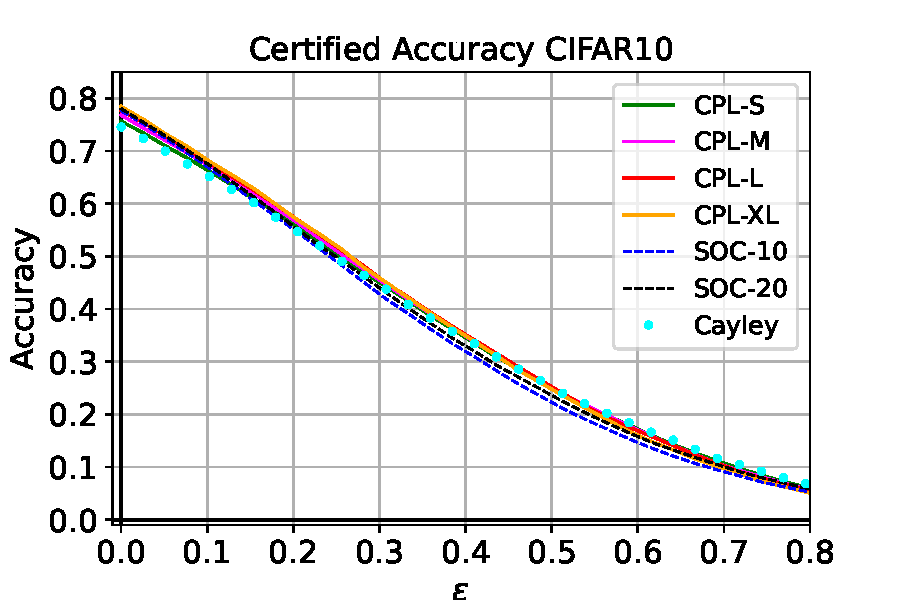
\includegraphics[width =0.48\textwidth]{sections/4_certification/images/cert_acc_eps_c10.pdf} & 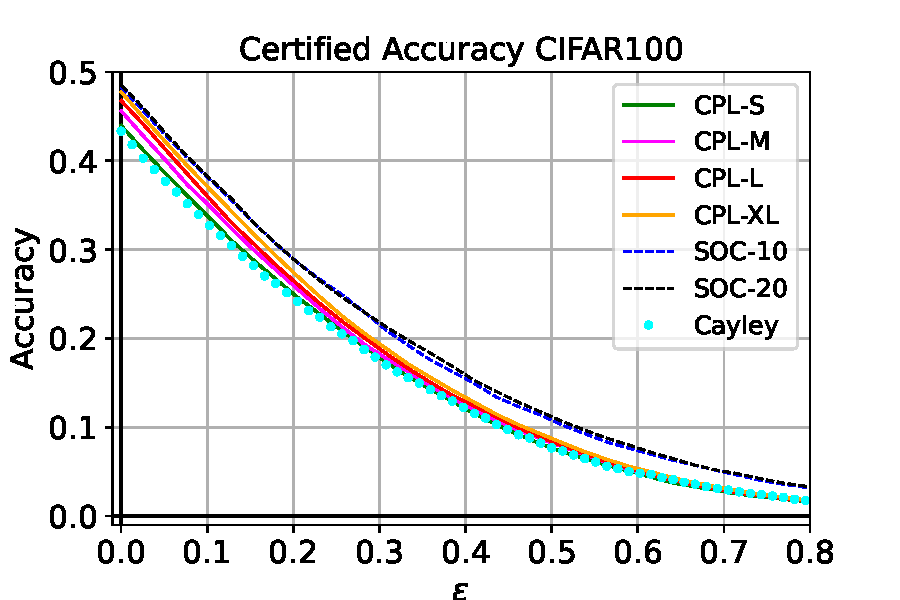
\includegraphics[width =0.48\textwidth]{sections/4_certification/images/cert_acc_eps_c100.pdf}
    \end{tabular}
    \caption{Certifiably robust accuracy  w.r.t. the perturbation $\varepsilon$ for our CPL networks and its concurrent approaches (SOC and Cayley models) on CIFAR10 and CIFAR100 datasets.}
    \label{fig:cert-acc}
\end{figure}

\paragraph{Certified Adversarial Robustness.} 
Results on CIFAR10 and CIFAR100 dataset are reported respectively in Tables~\ref{table:c10-comp} and~\ref{table:c100-comp}. We also plotted certified accuracy w.r.t. $\varepsilon$ on Figure~\ref{fig:cert-acc}. On CIFAR10, our method outperforms the concurrent approaches in terms of standard and certified accuracies for every level of $\varepsilon$ except SOC+ that uses additional tricks we did not use. On CIFAR100, our method performs slightly under the SOC networks but better than Cayley networks. Overall, our methods reach competitive results with SOC and Cayley layers. 

Note that we observe a small gain using larger and deeper architectures for our models. This gain is less important as $\varepsilon$ increases but the gain is non negligible for standard accuracies. In term of training time, our small architecture (CPL-S) trains very fast compared to other methods, while larger ones are longer to train.


\begin{figure}[h]
    \centering
    \begin{tabular}{cc}
    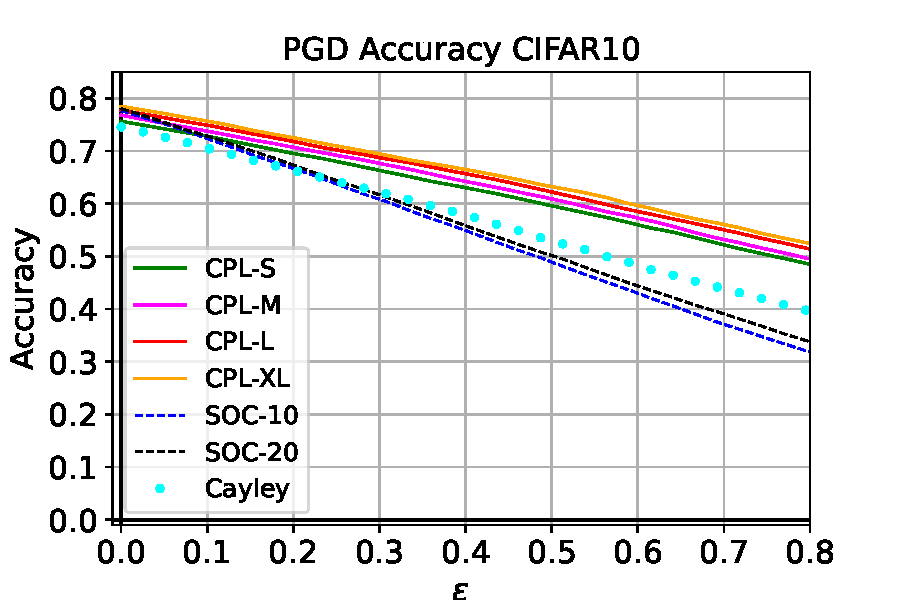
\includegraphics[width =0.48\textwidth]{sections/4_certification/images/pgd_acc_eps_c10.pdf} & 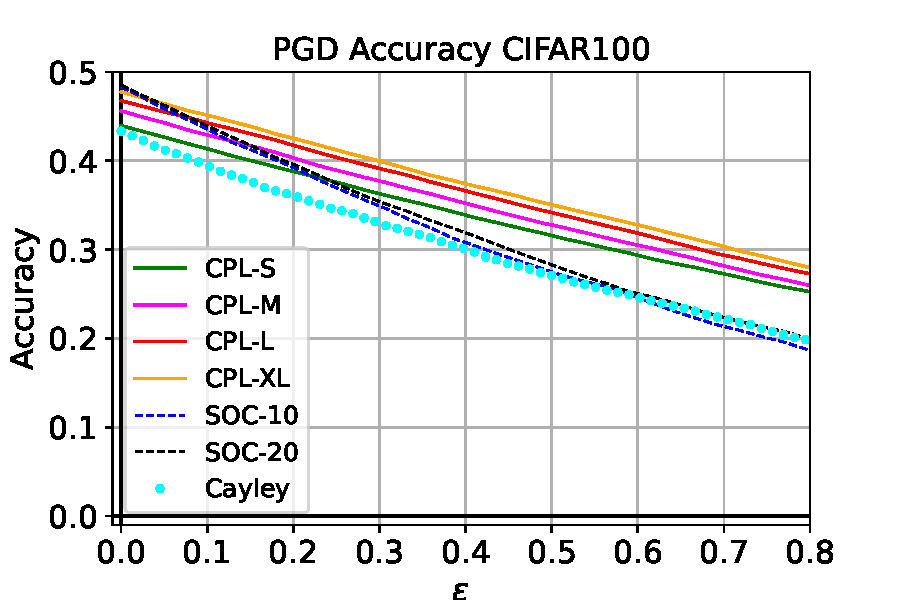
\includegraphics[width =0.48\textwidth]{sections/4_certification/images/pgd_acc_eps_c100.pdf}
    \end{tabular}
    \caption{Accuracy against PGD attack with 10 iterations w.r.t. the perturbation $\varepsilon$ for our CPL networks and its concurrent approaches on CIFAR10 and CIFAR100 datasets.}
    \label{fig:pgd-acc}
\end{figure}
\paragraph{Empirical Adversarial Robustness.} We also reported in Figure~\ref{fig:pgd-acc} the accuracy of all the models against PGD $\ell_2$-attack~\citep{kurakin2016adversarial,madry2018towards} for various levels of $\epsilon$. We used $10$ iterations for this attack. We remark here that our method brings a large gain of robust accuracy over all other methods. On CIFAR10 for $\varepsilon = 0.8$, the gain of CPL-S over SOC-10 approach is more than $10\%$. For CIFAR100, the gain is about $10\%$ too for $\varepsilon=0.6$. We remark that using larger architectures lead in a more substantial gain in empirical robustness. 

Our layers  only provide an upper bound on the Lipschitz constant, while orthonormal layers such as Cayley and SOC are built to exactly preserve the norms. This might negatively influence the certified accuracy since the effective Lipschitz constant is smaller than the theoretical one, hence leading to suboptimal certificates. This might explain why our method performs so well for empirical robustness tasks.






\begin{table*}[h]
  \centering
  \sisetup{%
    table-align-uncertainty=true,
    separate-uncertainty=true,
    detect-weight=true,
    detect-inline-weight=math
  }
  \begin{tabular}
  {
    l
    S[table-format=2.2]
    S[table-format=2.2]
    S[table-format=2.2]
    S[table-format=2.2]
    S[table-format=2.2]
    S[table-format=2.2]
  }
  \toprule
  &\multicolumn{1}{c}{\textbf{Batch}}& \multicolumn{1}{c}{\textbf{Standard Acc.}} & \multicolumn{3}{c}{\textbf{Provable Accuracy ($\varepsilon $)}} &  \multicolumn{1}{c}{\textbf{T./epoch (s)}} 
    \\
    \cmidrule{4-6}
    & \multicolumn{1}{c}{ } & \multicolumn{1}{c}{ } &\multicolumn{1}{c}{36/255} & \multicolumn{1}{c}{72/255} &  \multicolumn{1}{c}{108/255} & \multicolumn{1}{c}{\textbf{}} 
    \\
  \midrule
    \multirow{3}{*}{\textbf{CPL-S}} & 64 & 76.5& 62.9 & 47.3 & 32.0 & 48 \\
                                    & 128 & 76.1 & 62.8 & 47.1 & 32.3  & 31 \\
                                    & 256 & 75.6 & 62.3 & 46.9 & 32.2 & 22 \\
    \midrule
 \multirow{3}{*}{\textbf{CPL-M}} & 64 & 77.4 & 63.6 & 47.4 & 32.1  & 77 \\
                                    & 128 & 77.2 &63.5 & 47.5 & 32.1 & 50 \\
                                    & 256 & 76.8 & 63.2 & 47.4 & 32.4& 40 \\
    \midrule

 \multirow{3}{*}{\textbf{CPL-L}} & 64 & 78.4 & 64.2 & 47.8 & 32.2  & 162 \\
                                    & 128 & 78.2 & 64.3 & 47.9 & 32.5 & 109 \\
                                    & 256 & 77.6 & 63.9 & 48.1 & 32.7& 93 \\
  \midrule
 \multirow{3}{*}{\textbf{CPL-XL}} & 64 & 78.9 & 64.2 & 47.2 & 31.2  & 271 \\
                                    & 128 & 78.9 & 64.2 & 47.5 & 31.8 & 198 \\
                                    & 256 &78.5 & 64.4 & 47.8 & 32.4& 163 \\

  \bottomrule
  \end{tabular}%
  \caption{Results on the CIFAR10 dataset on standard and  provably certifiable accuracies for different values of perturbations $\varepsilon$ on CPL (ours) models with various batch sizes. The average time per epoch in seconds is also reported in the last column. All the reported networks use Last Layer Normalization.}
  \label{table:c10-comp-bs}%
\end{table*}%



\begin{table*}[h]
  \centering
  \sisetup{%
    table-align-uncertainty=true,
    separate-uncertainty=true,
    detect-weight=true,
    detect-inline-weight=math
  }
  \begin{tabular}
  {
    l
    S[table-format=2.2]
    S[table-format=2.2]
    S[table-format=2.2]
    S[table-format=2.2]
    S[table-format=2.2]
    S[table-format=2.2]
  }
  \toprule
  &\multicolumn{1}{c}{\textbf{Batch}}& \multicolumn{1}{c}{\textbf{Standard Acc.}} & \multicolumn{3}{c}{\textbf{Provable Acc. ($\varepsilon $)}} &  \multicolumn{1}{c}{\textbf{T./epoch (s)}} 
    \\
    \cmidrule{4-6}
    & \multicolumn{1}{c}{ } & \multicolumn{1}{c}{ } &\multicolumn{1}{c}{36/255} & \multicolumn{1}{c}{72/255} &  \multicolumn{1}{c}{108/255} & \multicolumn{1}{c}{\textbf{}} 
    \\
  \midrule
  \multirow{3}{*}{\textbf{CPL-S}} & 64 & 45,6 & 30,8 & 19,3 & 11,2 & 47 \\
                                    & 128 & 44,9 & 30,7 & 19,2 & 11,0 & 31\\
                                    & 256 & 44,0 & 29,9 & 19,1 & 10,9 & 23\\
  \midrule
  \multirow{3}{*}{\textbf{CPL-M}} & 64 & 46.6 & 31,6 & 19,6 & 11,6 & 78 \\
                                    & 128 & 46.3 & 31,1 & 19,7 & 11,5 & 55 \\
                                    & 256 & 45.6 & 31,1 & 19,3 & 11,3 & 41 \\

  \midrule

  \multirow{3}{*}{\textbf{CPL-L}} & 64 & 48.1 & 32,7 & 20,3 & 11,7 & 163 \\ 
                                    & 128 & 47,4 & 32,3 & 20,0 & 11,8 & 116 \\ 
                                    & 256 & 46,8 & 31,8 & 20,1 & 11,7 & 95 \\ 
  \midrule
  \multirow{3}{*}{\textbf{CPL-XL}} & 64 & 49,0 & 33,7 & 21,1 & 12,0 & 293 \\
                                    & 128 & 48,0 & 33,7 & 21,0 & 12,1 & 209 \\
                                    & 256 &47,8 & 33,4 & 20,9 & 12,6 & 164 \\

  \bottomrule
  \end{tabular}%
  \caption{Results on the CIFAR100 dataset on standard and  provably certifiable accuracies for different values of perturbations $\varepsilon$ on CPL (ours) models with various batch sizes. The average time per epoch in seconds is also reported in the last column. All the reported networks use Last Layer Normalization.}
  \label{table:c100-comp-bs}%
\end{table*}%

\paragraph{Effect of Batch Size in Training.}
In Tables~\ref{table:c10-comp-bs} and~\ref{table:c100-comp-bs}, we tried three different batch sizes (64, 128 and 256) for training our networks on CIFAR10 and CIFAR100 datasets, we remark a gain in standard accuracy in reducing the batch size for all settings. As the perturbation becomes larger, the gain in accuracy is reduced and even in some cases we may loose some points in robustness.





\begin{figure}[h]
    \centering
    \begin{tabular}{cc}
    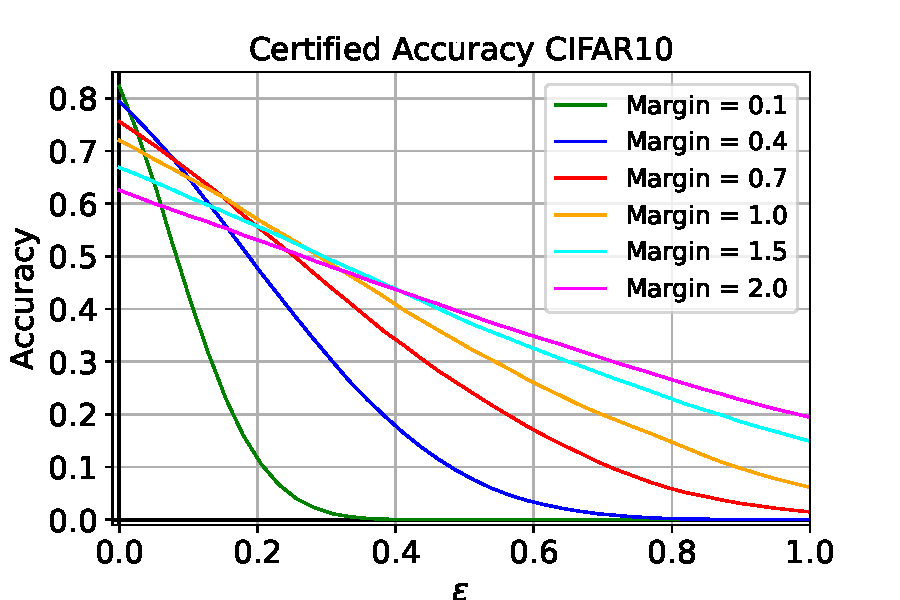
\includegraphics[width=0.48\textwidth]{sections/4_certification/images/cert_acc_margin_eps_c10.pdf}&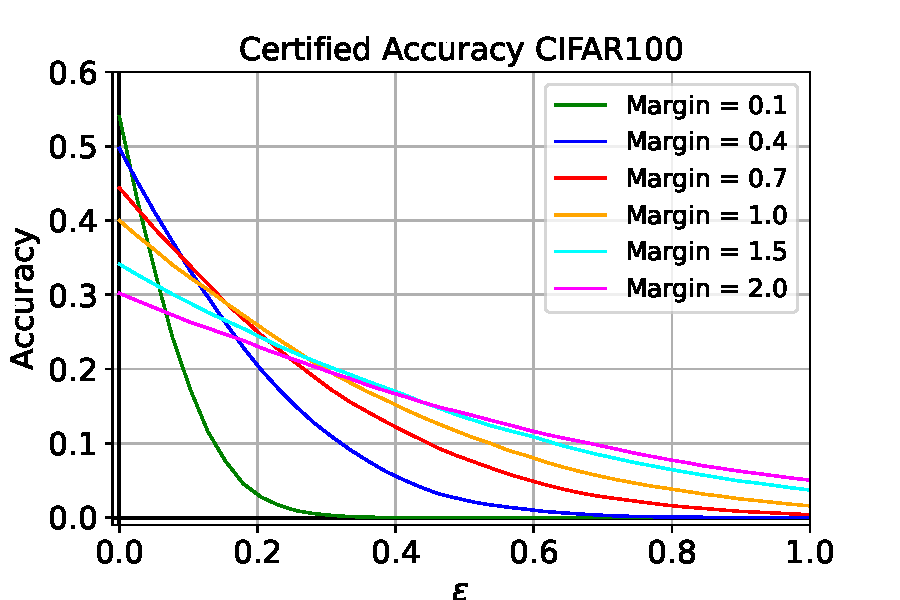
\includegraphics[width=0.48\textwidth]{sections/4_certification/images/cert_acc_margin_eps_c100.pdf}
    \end{tabular}
    \caption{Certifiably robust accuracy w.r.t. the perturbation $\varepsilon$ for our CPL-S  network with different margin parameters on CIFAR10 and CIFAR100 datasets.}
    \label{fig:cert-acc-margin}
\end{figure}


\begin{figure}[h]
    \centering
    \begin{tabular}{cc}
    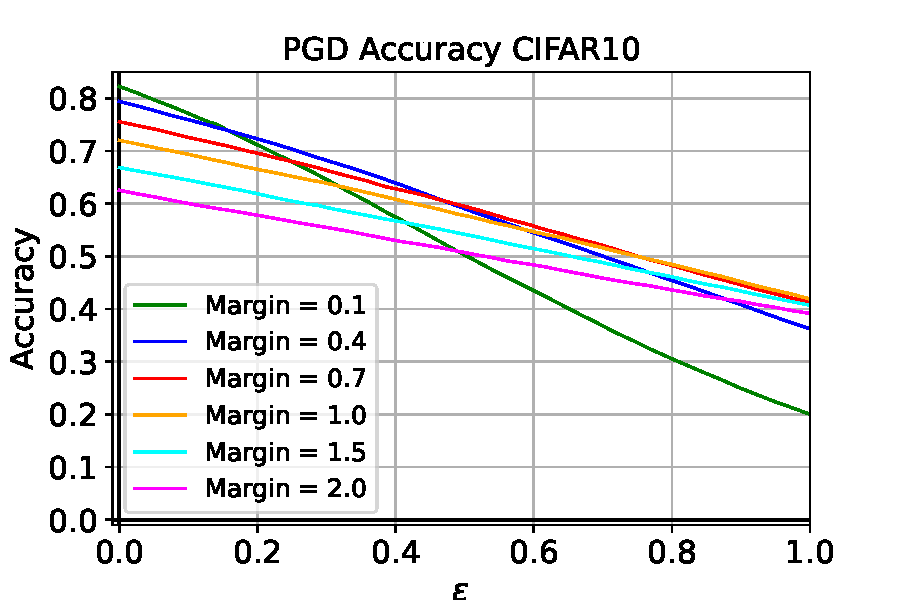
\includegraphics[width=0.49\textwidth]{sections/4_certification/images/pgd_acc_margin_eps_c10.pdf}&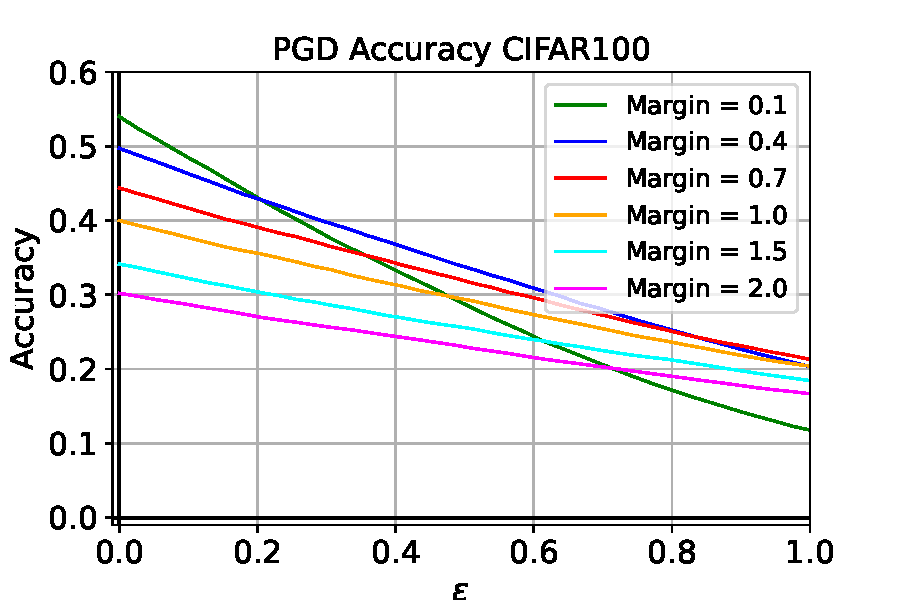
\includegraphics[width=0.49\textwidth]{sections/4_certification/images/pgd_acc_margin_eps_c100.pdf}
    \end{tabular}
    \caption{Certifiably robust accuracy w.r.t. the perturbation $\varepsilon$ for our CPL-S  network with different margin parameters on CIFAR10 and CIFAR100 datasets.}
    \label{fig:pgd-acc-margin}
\end{figure}

\paragraph{Effect of the Margin Parameter.}
In these experiments we varied the margin parameter in the margin loss in Figures~\ref{fig:cert-acc-margin} and~\ref{fig:pgd-acc-margin}. It clearly exhibits a tradeoff between standard and robust accuracy. When the margin is large, the standard accuracy is low, but the level of robustness remain high even for ``large'' perturbations. On the opposite, when the margin is small, we obtain a high standard accuracy but we are unable to keep a good robustness level as the perturbation increases. It is verified both on certified and empirical robustness.





\subsection{Training stability: scaling up to $1000$ layers}

\begin{figure}[h]
    \centering
    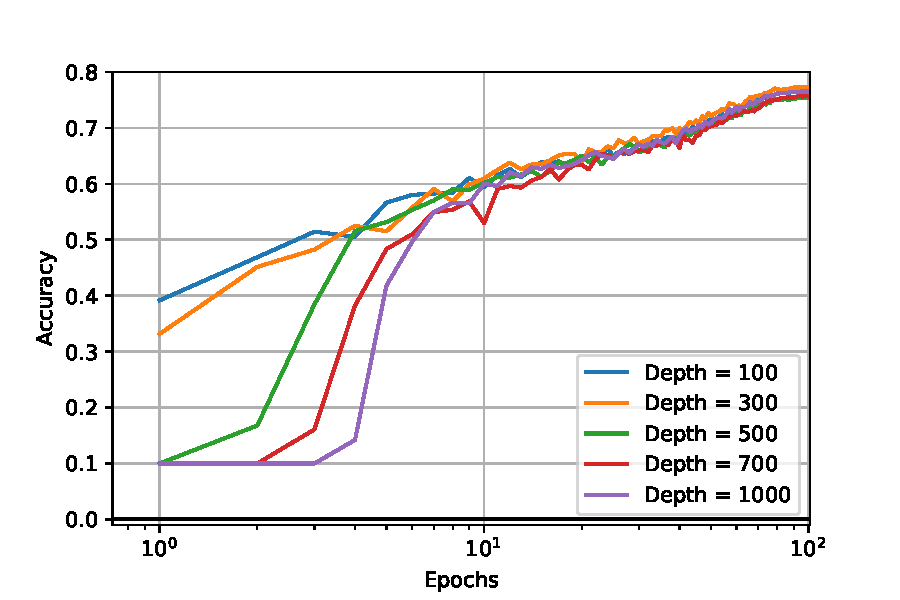
\includegraphics[width=0.5\textwidth]{sections/4_certification/images/final_cifar10_veryverydeep.pdf}
    \caption{Standard test accuracy w.r.t. the number of epochs (log-scale) for various depths for our neural networks ($100,300,500,700,1000$).}
    \label{fig:verydeep}
\end{figure}

While the Residual Network architecture limits, by design, gradient vanishing issues, it still suffers from exploding gradients in many cases~\citep{hayou2021stable}.
To prevent such scenarii, batch normalization layers~\citep{ioffe2015batch} are used in most Residual Networks to stabilize the training.

Recently, several works~\citep{miyato2018spectral,farnia2018generalizable} have proposed to normalize the linear transformation of each layer by their spectral norm.
Such a method would limit exploding gradients but would again suffer from gradient vanishing issues.
Indeed, spectral normalization might be too restrictive: dividing by the spectral norm can make other singular values vanishingly
small.
While more computationally expensive (spectral normalization can be done with $1$ Power Method iteration), orthogonal projections prevent both exploding and vanishing issues. 

On the contrary the architecture proposed  has the advantage to naturally control the gradient norm of the output with respect to a given layer.
Therefore, our architecture can get the best of both worlds: limiting exploding and vanishing issues while maintaining scalability. 
To demonstrate the scalability of our approach, we experiment the ability to scale our architecture to very high depth (up to 1000 layers) without any additional normalization/regularization tricks, such as Dropout~\citep{srivastava2014dropout}, Batch Normalization~\citep{ioffe2015batch} or gradient clipping~\citep{pascanu2013difficulty}.
With the work done by~\cite{xiao2018dynamical}, which leverage Dynamical Isometry and a Mean Field Theory to train a $10000$ layers neural network, we believe, to the best of our knowledge, to be the second to perform such training. 
For the sake of computation efficiency, we limit this experiment to architecture with $30$ feature maps.
We report the accuracy in terms of epochs for our architecture in Figure~\ref{fig:verydeep} for a varying number of convolutional layers.
It is worth noting that for the deepest networks, it may take a few epochs before the start of convergence.
As \cite{xiao2018dynamical}, we remark there is no gain in using very deep architecture for this task.


\subsection{Relaxing linear layers}

\begin{table*}
\begin{tabular}{lrrr}
\toprule
  & \multicolumn{1}{c}{\textbf{h = 1.0}} & \multicolumn{1}{c}{\textbf{h = 0.1}} & \multicolumn{1}{c}{\textbf{h = 0.01}} \\
\midrule
\textbf{Standard} & 85.10 & 82.23 & 78.53 \\
\textbf{PGD ($\varepsilon = 36/255$}) & 61.45 & 62.99 & 60.98 \\
\bottomrule
\end{tabular}
\caption{Level of accuracy of CPL networks when the constraints on the step-size is relaxed. We fixed the step-size $h$ to different values and measured standard and empirically robust accuracy. Here the CPL-M model is used.}
\label{table:relaxstep}
\end{table*}

Table~\ref{table:relaxstep} shows the result of the relaxed training of our CPL architecture, i.e. we fixed the step $h_t$ in the discretized convex potential flow of Proposition~\ref{prop:discrete_convex_potentials}.
Increasing the constant $h$ allows for an important improvement  in the standard accuracy, but we loose in robust empirical accuracy.
While computing the certified accuracy is not possible in this case due to the unknown value of the Lipschitz constant, we can still notice that the training of the network are still stable without normalization tricks, and offer a non-negligible level of robustness. 



